%%%%%%%%%%%%%%%%%%%%%%%%%%%%%%%%%%%%%%%%%%%%%%%%%%%%%%%%%%%%%%%%%%%%%%%%%%%%%%%%
%2345678901234567890123456789012345678901234567890123456789012345678901234567890
%        1         2         3         4         5         6         7         8

\documentclass[letterpaper, 10 pt, conference]{ieeeconf}  % Comment this line out
                                                          % if you need a4paper
%\documentclass[a4paper, 10pt, conference]{ieeeconf}      % Use this line for a4
                                                          % paper

\IEEEoverridecommandlockouts                              % This command is only
                                                          % needed if you want to
                                                          % use the \thanks command
\overrideIEEEmargins
% See the \addtolength command later in the file to balance the column lengths
% on the last page of the document

\usepackage{graphicx}

% The following packages can be found on http:\\www.ctan.org
%\usepackage{graphics} % for pdf, bitmapped graphics files
%\usepackage{epsfig} % for postscript graphics files
%\usepackage{mathptmx} % assumes new font selection scheme installed
%\usepackage{times} % assumes new font selection scheme installed
%\usepackage{amsmath} % assumes amsmath package installed
%\usepackage{amssymb}  % assumes amsmath package installed

\title{\LARGE \bf
Web Information Retrieval - Final Project
}

\author{Angelo Catalani, Valerio Colitta and Alessandro Lo Presti}% <-this % stops a space


\begin{document}



\maketitle
\thispagestyle{empty}
\pagestyle{empty}


%%%%%%%%%%%%%%%%%%%%%%%%%%%%%%%%%%%%%%%%%%%%%%%%%%%%%%%%%%%%%%%%%%%%%%%%%%%%%%%%
\begin{abstract}

This projects is inspired by \cite{c1}. We introduce a new semantic similarity function and provide the code that implements the GVSM cosine similarity and all the APIs to test a generic semantic similarity function


\end{abstract}


%%%%%%%%%%%%%%%%%%%%%%%%%%%%%%%%%%%%%%%%%%%%%%%%%%%%%%%%%%%%%%%%%%%%%%%%%%%%%%%%
\section{INTRODUCTION}

The vector space model is characterized by the representation of documents and queries as vectors and the cosine similarity to compute the similarity score between them.\\This means that if the distinct terms in a given collection are n, each document is a n-dimensional vector.\\The VSM assumes that for each term $t_i$ there exists a vector $\vec{t_i}$ in the vector space the represents it, and these vectors form the space basis.\\This leads to the fact, each document (or query) is a linear combination of the vectors $t_i$ : $\vec{d_k} = \sum\limits_{i=1}^n w_i\vec{t_i}$ , where $w_i$ is the tf-idf score for the term $t_i$ in the document : $d_k$  .\\The underlying assumption is the pairwise orthogonality of terms vector that brings to the conclusion there can not be any semantic correlation between terms.\\The GVSM extends the VSM by non considering terms vectors orthogonal and computing the similarity score between terms according the following formula : 
\begin{equation}
    score(\vec{d},\vec{q}) = \frac{\mathop{\sum_{j=1}^{n'}\sum_{i=1}^{n'}}\vec{t_i}\cdot\vec{t_j}\cdot d[i]\cdot q[j] }{||\vec{d_k} ||\cdot||\vec{q} ||}
\end{equation}.\\It is interesting to note this formula reduces to the classical cosine similarity assuming pairwise orthogonality of the terms vectors because that product is always zero except when they are the same($i=j$).\\The dot product of the terms is their semantic correlation.
\section{Generalized Vector Space Model}
The paper\cite{c1} taken into consideration, considered documents to be $n' = n\cdot(n-1)/2$ dimensional vectors where, each dimension stands for a distinct pair of terms and all the distinct terms are $n$.\\In particular for a given document $d_k$, the entry
\begin{equation}
    d_k[i][j] = d_k(t_i,t_j) = (tf-idf(t_i,d_k)+tf-idf(t_j,d_k)) \cdot \vec{t_i}\cdot\vec{t_j}
\end{equation}.\\The dimension is not $n*n$ because it is assumed the similarity function between terms is symmetric, so that the entry  $d_k(t_i,t_j) = d_k(t_j,t_i)$.\\Finally, the score function has been defined as :
\begin{equation}
    score(\vec{d},\vec{q}) = \frac{\mathop{\sum_{j=1}^{n'}\sum_{i=1}^{n'}}d_k[i][j]\cdot q[i][j] }{||\vec{d_k} ||\cdot||\vec{q} ||}
\end{equation}
\section{A new semantic similarity function}
To tackle semantic similarity among terms, we relied on \textbf{WordNet®}\cite{c5}, a large lexical database of English. Nouns, verbs, adjectives and adverbs are grouped into sets of cognitive synonyms (synsets), each expressing a distinct concept. Synsets are interlinked by means of conceptual-semantic and lexical relations.
.\\
We decided to take into consideration only the \texttt{hypernym-relationships} to determine words similarity. The key point was to find the \texttt{Lowest Common Ancestor} (LCA) in the WORDNET hypernym tree. It specifies the lowest parent two senses have in common.\\
Intuitively, the deeper the LCA, the stronger the similarity. This is true, but also the distance between the two terms is important.\\
If two pairs of terms meet at the same LCA, it does not mean they are identical in the similarity. If they live on two separate branches, then they are not so similar, and this should be taken into account.\\
This is why we introduced another metric, we called \texttt{Path Distance} (PD), which is the length of the path from \texttt{t$_1$} to \texttt{t$_2$} in the tree (for this one, the longer, the worse).\\
Finally our similarity measure is composed of two elements
\begin{itemize}
\item PD : Path Distance
\item LCAD : Lowest Common Ancestor Depth
\end{itemize}
Given two terms, for each pair of senses we compute
\begin{equation}
CSIM(s_1,s_2) = \frac{1}{\sqrt{PD+1}} \times \log(LCAD)
\end{equation}
We added the square root to the first term of the equation, in order to smooth it out. We did the same for the second one.
At the end
\begin{equation}
CSIM(t_1,t_2) = \max_{(s_i,s_j)} CSIM(s_i,s_j)
\end{equation}
This turns out to work well also to measure the non-similarity, in fact suppose that two terms have a small \texttt{PD} because they are close each other, but live near the root of the tree. In this case, \texttt{LCAD} will lower the similarity.\\
\subsection{Complexity}
This similarity measure performs better (wrt to complexity) than the one proposed by \cite{c1}, that implements a shortes path that has complexity $O((E+N)\log(N)$, while the one proposed in this project has to compute the lowest common ancestor that has complexity $O(N))$. The only bottleneck may be the log and sqrt operations, but their argument are bound to be at most $2N$.
\section{The Dataset}
\subsection{Document - Query dataset}
We wanted to replicate the experiments made in the paper, but the \texttt{TREC} dataset was not available for free, so we selected the NPL dataset \cite{c2}.\\
The NPL (also known as the VASWANI) collection is a collection of around 10,000 document titles. It has a bit of a reputation of messing up people's experiments.\\
Together with those 10,000 documents, there are 93 queries, each of those with the top relevant documents ranked manually.\\
In particular, we have:
\begin{itemize}
    \item Documents: \texttt{11429}
    \item Queries: \texttt{93}
    \item Distinct Terms: \texttt{11945}
\end{itemize}
\subsection{Term-Term dataset}
To evaluate the semantic similarity function, according to a golden standard, we used the same documents adopted by the paper. It is a set of tuples $<c_i, c_j, s_ij>$, where $c_i, c_j$ are terms, and $s_{ij}$ is their similarity obtained from by human judgment.\\
The quality of a semantic similarity measure is assessed with Spearman correlation between the similarity scores of humans and a measure. This evaluation directly assesses performance of the measure and indirectly assesses quality of relation extraction with the measure.\\
We use three standard human judgments datasets MC (Miller and Charles, 91), RG (Rubenstein and Goodenougth, 1965) and WordSim353 (Finkelstein et al., 2001) composed of 30, 65, and 353 pairs of terms respectively.
\section{Implementation and choices}
Having limited computational resources, tests have been conducted after resizing the dataset. We trimmed down the set of documents to a subset of about $2000$, which are all the documents assessed as relevant by a human being for each query. This means that in any case, when testing the function for a given query, its relevant documents will be there.\\
Of course this was done only during the testing phase. The \texttt{tf-id} computation has been done on all the $11429$ documents.\\
We wanted to make a comparison also against the traditional VSM, so for each document and query, we computed the cosine similarity.\\
To compare both the methods we adopted the standard \texttt{precision-recall} plot.
It is calculated as an average of the precision for a given recall level for the number  query considered .\\In particular 10 recall levels have been considered : $ 0.1, 0.2, ... , 1.0 $.\\ \\
Another trick to speed up the computation was to approximate the score function, by considering the union of the terms of both the document and the query, instead of using the whole term vector in a double nested loop. That just wouldn't make the computation end.\\
%By using the union of the terms, we have the same numerator of the original query, but a different, smaller denominator. 
%In addition to this, it has been executed a test also on the classical cosine similarity where it has been possible to consider the whole dataset since each computation has a linear complexity.%
\section{Performance}
The performance will be divided into two categories, one for each kind of dataset.
\subsection{Term-Term performance}
This first part focuses on the capability of the semantic similarity measures to grasp the closeness of terms. We use the three datasets specified above and for each semantic similarity function taken into account, we compute the Spearman correlation coefficient.\\
We use the similarity function specified by the paper (SR) \cite{c1}, our custom function (CSIM), the Wu-Palmer (WUP) \cite{c3} function, the Leacock-Chodorow Similarity (LCH) \cite{c4} and the Path similarity (PS).\\   \\
Surprisingly, our custom similarity, overall, performs better (both in terms of time and score) than the \cite{c3} \cite{c4} and PS. However, it is below \cite{c1}. The lower complexity probably paid for the lower score.
\begin{table}[h]
\centering
\begin{tabular}{l|l|l|l|l|l}
     & LC   & WP   & PS   & SR   & \textbf{CSIM} \\ \hline
R\&G & 0.75 & 0.78 & 0.78 & 0.86 & \textbf{0.76} \\ \hline
M\&C & 0.74 & 0.72 & 0.72 & 0.85 & \textbf{0.77} \\ \hline
WS   & 0.33 & 0.29 & 0.29 & 0.61 & \textbf{0.34}
\end{tabular}
\end{table}
\subsection{Document-Query Performance}
As we earlier, we wanted to compare how well both the VSM and the GVSM performed.\\
For the GVSM, because of too much computational need, we decided to interpolate the precision-recall plot only for a subset of queries.\\
\multicolfloat{1}{2}{\centering
                     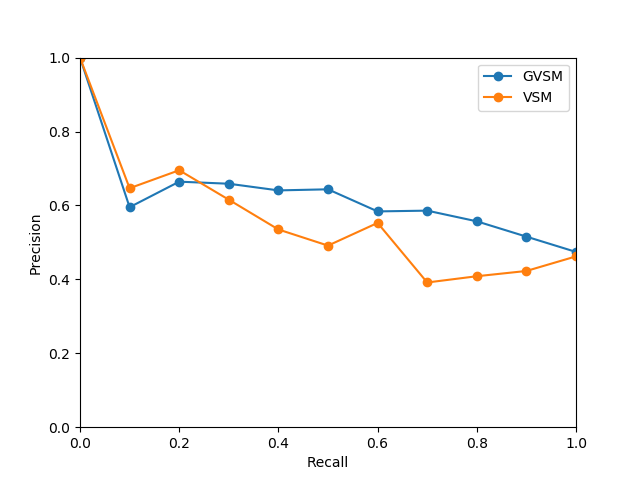
\includegraphics[width=9cm]{Plot_overlap.png}
                    }\\
As expected the GVSM performs better than the standard one by at least $10\%$. It is an encouraging results, but it took us more than 2 hours just to rank 30 queries\dots We don't know what the results would be on a more powerful machine, with a more optimized code, but surely it will not beat the speed of a scalar product.
\section{Conclusions}
\subsection{Thoughts about the GVSM}
As it can be seen from the previous sections, the concept of semantic similarity is surely a better choice over the simple cosine similarity. The real problem is the time-demanding operation for computing the $(t_i,t_j)$ score. We don't think this approach can be used efficiently at run-time. 
\subsection{Future Work}
In order to make the score function faster, each computation could be done in a multithreading context.\\In addition to this the term-to-term similarity scores could be precomputed and stored in a global dictionary.\\ \\
Another future goal is to extend the function also to adjectives, since most of the similarity functions do not work with them, because they lack hypernyms. We tried to integrate them in our function during initial development, but found some difficulties with converting an adjective to a noun in wordnet. But it can be done, with some amount of work.
\begin{thebibliography}{99}

\bibitem{c1} George Tsatsaronis and Vicky Panagiotopoulo,
  \emph{ A Generalized Vector Space Model for Text Retrieval Based on Semantic Relatedness}.
  \\Department of Informatics Athens University of Economics and Business, 76, Patision Str., Athens, Greece,
  2009\\
\bibitem{c2} NPL Collection, http://ir.dcs.gla.ac.uk/resources/test$_$collections/npl/ \\
\bibitem{c3} Wu Z. and Palmer M.
 \emph{Verbs semantics and lexical selection}.
 \\Proceedings of the 32nd annual meeting on Association for Computational Linguistics\\
\bibitem{c4}Leacock, Claudia and Miller, George A and Chodorow, Martin
\emph{Using corpus statistics and WordNet relations for sense identification}\\
Computational Linguistics
\bibitem{c5}WordNet, https://wordnet.princeton.edu/
\end{thebibliography}




\end{document}
